\documentclass[11pt, a4paper]{scrartcl}

\usepackage[left=3cm, right=3cm, top=3cm, bottom=3cm]{geometry}
\usepackage{graphicx}
\usepackage{array}
\usepackage{amsmath}


\newcommand{\git}{\mathbin{
  \mathchoice{/\mkern-6mu/}% \displaystyle
    {/\mkern-6mu/}% \textstyle
    {/\mkern-5mu/}% \scriptstyle
    {/\mkern-5mu/}}}% \scriptscriptstyle


\title{Monte Carlo Methods - Sheet 3}
\subtitle{Ising Model: Autocorrelation and error estimation}
\author{Tobias Sizmann}

\begin{document}
\maketitle
\textit{You want to build a nuclear reactor. You do a Monte Carlo simulation of the reaction. It looks fine. You are not so easily satisfied. You estimate the error on the results. Still looks fine. You build the reactor. You start it. Boom. You forgot autocorrelation.}
\section{Introduction}
    Writing a simulation that returns a result is not necessarily a difficult task. But a simulation alone is not sufficient for answering real world questions. One needs to estimate an upper bound of error on the result. And ideally this upper bound should be as low as possible - it should reflect the true standard error in the statistical sense. Of course every simulation has an underlying model and therefore additional systematic errors per definition, but for now we want to focus on the statistical aspect. Here two challenges will arise. First challenge will be to deal with autocorrelation. Huge autocorrelations in a sample effectively reduce the number of statistically independent configurations and therefore increase the standard error. We will find a method to calculate the autocorrelation and determine how many steps configurations need to be apart for them to be independent. The second challenge will be estimation of error on secondary quantities. To this end we will use three different methods and compare their results to determine which method is suitable for which case. (I am wondering as to why jackknife is not done here. Isn't this like the go-to method in all of lattice QCD?)
\section{Autocorrelation and error estimation on primary quantities}
\subsection{Autocorrelation function}
    \begin{figure}
        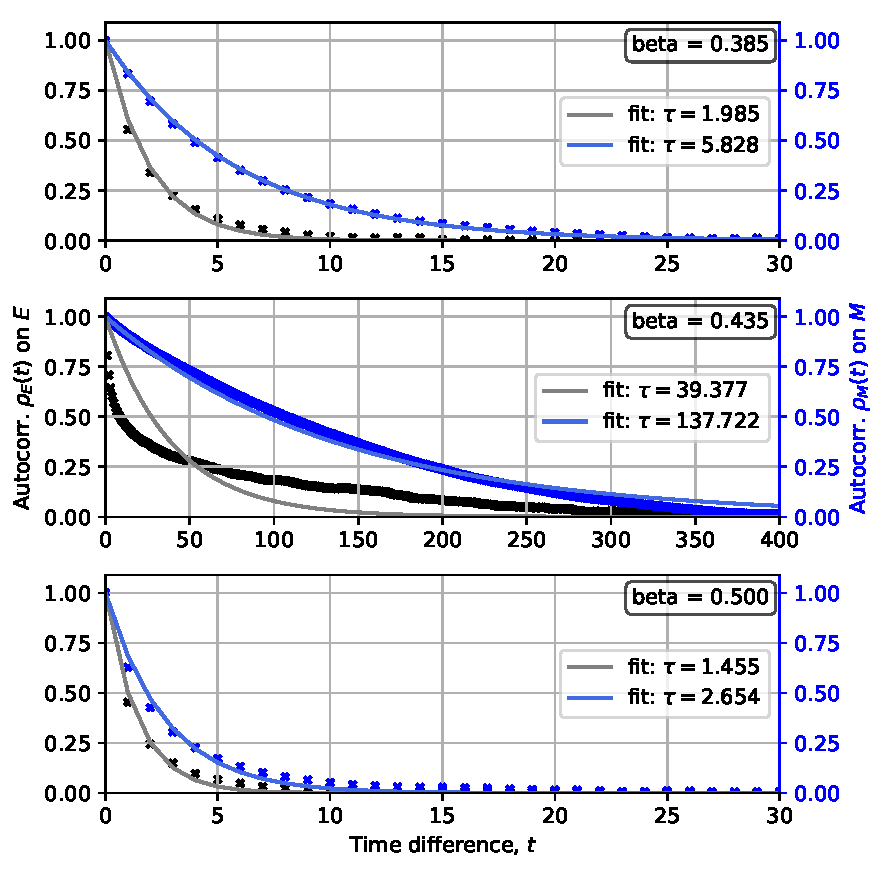
\includegraphics{autocorrelations.pdf}
        \label{fig1}
        \caption{\textbf{Autocorrelation of Markov chains |}  For temperatures $T = 2.0, 2.3, 2.6$ three chains were generated using the Metropolis algorithm on a 64x64 grid. Plotted are the autocorrelation functions for energy density (black) and magnetisation density (blue) for each respective temperature. An exponential decay of the form $\exp(-\frac{t}{\tau})$ has been fitted (gray / light blue) to measure autocorrelation time.}
    \end{figure}
    As already motivated we need to find a measure of correlation of samples seperated by some number of steps $t$. To this end, one can define the autocovariance function $C_y(t)$ on some primary quantity $y$, which emerges naturally if one tries to find a correction of the error estimate for correlated Markov chains:
    $$C_y(t) = \sum_{i = 1}^{N-t} \langle (y_i - \bar{y})(y_{i+t} - \bar{y}) \rangle$$
    The expectation values can be estimated on a sample. It is important to note that for increasingly large $t$ the estimate has an increasingly larger error since the number of configurations to be summed over becomes smaller. With this, one can define the autocorrelation function
    $$
    \rho_y(t) = \frac{C_y(t)}{C_y(0)} = \frac{C_y(t)}{\sigma_y^2} .
    $$
    In figure \ref{fig1} the autocorrelation functions of energy density $E$ and absolute magnetisation density $M$ have been calculated and plotted for three different samples with temperatures $T = 2.0, 2.3, 2.6$, respectively. They exhibit an exponential decay (to be precise: it's a sum of exponential decays) and fit with $f(x) = \exp(-\frac{t}{\tau})$ has been done. $\tau$ will be our measure for the length of correlations in the chain. We will see another way to extract an approximation for $\tau$ later. Note, that the autocorrelation for $T = 2.3$ (i.e. $\beta = 0.435$) for both the energy and magnetisation is larger by several orders of magnitude. This phenomenon is called critical slowing down and appears whenever a chain is being generated for parameters close to a critical point. It is an intrinsic property of local update algorithms like the Metropolis algorithm. Also note that the fits work out nicely except for the energy density at a temperature of $T = 2.3$. Here is becomes apparent that the autocorrelation function is truely described by a sum of exponential decays.

\subsection{Error on correlated samples}
    To estimate the error on a primary quantity $\sigma_{\bar{y}}$ on can use the following formula:
    $$\sigma_{\bar{y}} = \frac{\sigma_y}{\sqrt{N}}$$
    This requires the configurations to be statistically independent. However, if one is using - for example - the Metropolis algorithm to generate the samples, they are inherently correlated. Therefore, one needs to find how many steps of seperation are required for two configurations to not be correlated anymore. To this end, one can calculate the integrated autocorrelation time $\tau_{int}$. It naturally emerges when taking autocorrelations into account. Configurations are then assumed to be independent if they have a seperation of $2 \tau_{int}$, i.e. the effective number of configurations is $N / (2 \tau_{int})$ and the above formula needs to be adjusted accordingly:
    $$\sigma_{\bar{y}} = \frac{\sigma_y}{\sqrt{N / (2 \tau_{int})}} = \sqrt{\frac{2 \tau_{int}}{N}}\sigma_y$$
    Here, $\tau_{int}$ can be calculated from the chain itself by the following formula:
    $$\tau_{int} = \frac{1}{2} + \sum\limits_{\substack{t\ge1 \\ \mathrm{until}\ \rho(t) < 0}} \rho(t)$$
    The somewhat weird condition "$\mathrm{until}\ \rho(t) < 0$" deals with the aforementioned fluctuations of the autocorrelation function $\rho(t)$ for large $t$. In the following table the autocorrelation times extracted by fitting $\tau_{fit}$ (see fig. \ref{fig1}) are compared with the integrated autocorrelation times $\tau_{int}$ evaluated on the same chains.
    \begin{center}
    \begin{tabular}{|c||c|c||c|c|}
        \hline
        Temp. $T$ & $\tau_{E, int}$ & $\tau_{E, fit}$ & $\tau_{M, int}$ & $\tau_{M, fit}$ \\
        \hline
        \hline
        2.0 & 1.78 & 1.45 & 3.07 & 2.65 \\
        \hline
        2.3 & 51.05 & 39.38 & 131.65 & 137.72 \\
        \hline
        2.6 & 2.28 & 1.98 & 5.88 & 5.83 \\
        \hline
    \end{tabular}
    \end{center}
    One can see that fitted and integrated autocorrelation times agree up to a difference of maximally $25\%$. We can therefore conclude that the integrated autocorrelation time is a sufficient estimate for the correction of errors. One can finally calculate the error on the estimates of energy density and magnetisation density according to $\sigma_{\bar{y}} = \sqrt{2\tau_{int}N^{-1}}\sigma_y$. This yields the following results:
    \begin{center}
    \begin{tabular}{|c||c|c|}
        \hline
        Temp. $T$ & $\bar{E} \pm \sigma_{\bar{E}}$ & $\bar{M} \pm \sigma_{\bar{M}}$ \\
        \hline
        \hline
        2.0 & $-1.745242 \pm 0.000160$ & $0.911141 \pm 0.000108$ \\
        \hline
        2.3 & $-1.354763 \pm 0.001692$ & $0.425283 \pm 0.010415$ \\
        \hline
        2.6 & $1.028587 \pm 0.000231$ & $0.074932 \pm 0.000604$ \\
        \hline
    \end{tabular}
    \end{center}
    Note how the errors around the critical point $T = 2.3$ are larger by one up to two orders of magnitude. This has two reasons. First, the variance of energy density and magnetisation density increase around the critical point. This is a property of the Ising Model and cannot be avoided without changing the model itself. Secondly, the aforementioned critical slowing down comes into play, effectively increasing the autocorrelation times and therefore reducing the number of statistically independent configurations. This is a property of the sample generation algorithm and can be dealt with by choosing a better algorithm.


\section{Errors on secondary quantities}
    Due to the structure of secondary quantities a standard error cannot be evaluated in the same way as for primary quantities. Several methods have been developed to estimate the error on secondary quantities, which will also deal with the effects of autocorrelation. We will apply these methods to calculate the error on the heat capacity density and magnetic susceptibility density.
\subsection{Error propagation}
    This method assumes that fluctuations around the means of the primary quantities the secondary quantity is dependent on are small and one can approximate in first order leading to a effective primary quantity. These read for our case of heat capacity density $c$ and magnetic susceptibility density $\chi$:
    $$
    c_{eff} = \beta ^ 2 L ^ 2 (E^2 - 2 \bar{E} E)
    $$
    $$
    \chi_{eff} = \beta L ^ 2 (M^2 - 2 \bar{M} M)
    $$
    One can then proceed to calculate the error using the procedure developed in Section 2. This approach however is bound to fail when the fluctuations of $E$ and $E^2$ become so large that approximation in first order is not justified. This might be the case for temperatures close to the critical point.
\subsection{Blocking method}
    This method directly works with the definition of the standard error. One divides the Markov chain into even blocks and evaluates the secondary quantity on each of these blocks. Then one can calculate the variance over all blocks and retrieve an estimation of the error on the complete chain. The autocorrelation does not need to be taken into account explicitly here. There is a caveat to this, however. If the autocorrelation time becomes so large that one blocks does not contain a sufficient amount independent configurations, the error estimate becomes smaller than it truely is. Reducing the number of blocks might not be an option either if the chain itself is not long enough.
\subsection{Bootstrap method}
    The idea of this method is to resample the given chain and create several new samples this way. The secondary quantity can then be evaluated on each respective sample and the variance of the resulting values leads to an estimation of the error. Autocorrelation must be taken into account explicitly. To this end one calculates the autocorrelation time $\tau$ of the chain on some primary quantity (energy for heat capacity and magnetisation for magnetic susceptibility) and only takes every $2\tau$-th configuration into account for resampling. By doing this, one can guarantee that the configurations in the new samples are statistically independent. This method will not artifically decrease the error estimate close to the critical point. Note however, that there is some ambiguity in the choice of the primary quantity to calculate the autocorrelation time on. To ensure statistic independence one would choose the primary quantity with the highest autocorrelation time. This might lead to overestimation of the error, though. For example, assume as a simple extreme case the following secondary quantity $f(\mu_x,\mu_y) = \mu_x + 0.0000001 * \mu_y$. It is intuitive that if the error on $\mu_y$ is even several magnitudes larger (for example by larger autocorrelation times) than the error on $\mu_x$, it should not affect the error on the secondary quantity $f$ much. Therefore one can conclude, that using the largest autocorrelation time of the primary quantities that the secondary quantity is dependent on results in an upper bound of error but might largely differ from the actual error.
\subsection{Results}
    The error estimates using all 3 methods are shown in the following table. The values are calculated for chains generated by the Metropolis algorithm on a 64x64 grid:
    \begin{itemize}
        \item T = 2.0
        \item[ ]
            \begin{tabular}{|c||c|c|}
            \hline
            Method & $\sigma_c$ & $\sigma_\chi$ \\
            \hline
            \hline
            Propagation & 0.004413 & 0.005333 \\
            \hline
            Blocking & 0.002975 & 0.004451 \\
            \hline
            Bootstrap & 0.006701 & 0.005934 \\
            \hline
            \end{tabular}
        \item T = 2.3
        \item[ ]
            \begin{tabular}{|c||c|c|}
            \hline
            Method & $\sigma_c$ & $\sigma_\chi$ \\
            \hline
            \hline
            Propagation & 0.036158 & 2.398757 \\
            \hline
            Blocking & 0.032023 & 2.858065 \\
            \hline
            Bootstrap & 0.092392 & 3.940361 \\
            \hline
            Multiple chains & 0.029870 & 2.912681 \\
            \hline
            Corr. bootstrap & 0.036629 & 2.500663 \\
            \hline
            \end{tabular}
        \item T = 2.6
        \item[ ]
            \begin{tabular}{|c||c|c|}
            \hline
            Method & $\sigma_c$ & $\sigma_\chi$ \\
            \hline
            \hline
            Propagation & 0.004600 & 0.077597 \\
            \hline
            Blocking & 0.005895 & 0.103591 \\
            \hline
            Bootstrap & 0.007045 & 0.088420 \\
            \hline
            \end{tabular}
    \end{itemize}
    One can see that the values generally agree in order of magnitude across all methods. Interestingly at the critical point $T = 2.3$ the Bootstrap method returns a much larger error on the heat capacity than the other two methods. We know that at the critical point the error propagation method and the blocking method might underestimate the error, while the bootstrap method might overestimate the error. In order to investigate this further, 100 thermalized Markov chains with the same parameters (64x64 grid, 90000 sweeps, $T = 2.3$) but different seeds have been generated and the error has been calculated as standard deviation of the heat capacity over these 100 chains. The results are also shown in the table above (denoted as multiple chains). Here it becomes apparent, that the bootstrap method is largely overestimating the error. One possible way to fix this is to use the autocorrelation time on the effective primary quantity (see Sec. 3.1) for the selection of independent configurations. The results are also shown in the above table (denoted as corrected bootstrap). As one can see, this greatly improves the quality of the estimate.

\end{document}
